
\chapter{Implementazione} 

In questo capitolo si descrivono e si motivano le scelte progettuali
realizzate nell'implementazione dell'applicazione, soffermandosi in
particolar modo sulle migliorie apportate al programma di partenza.
Sono inoltre descritti due esercizi rappresentativi \ref{sec:Esempi},
per spiegare brevemente l'utilizzo dell'applicazione da parte degli
studenti.


\section{Descrizione iniziale}

Il software realizzato si presenta allo studente con una schermata
iniziale contenente l'elenco degli esercizi preparati organizzati
tramite una struttura ad albero per argomenti. Selezionando un particolare
esercizio si visualizza nella parte inferiore della finestra una breve
descrizione dell'esercitazione.

Una volta scelta l'attività, allo studente si apre un'ulteriore finestra,
molto simile a quella del sistema Trakla2, ma con qualche integrazione,
di cui si parlerà in seguito in questo capitolo. In modo analogo al
sistema di esercizi originale, l'utente deve simulare il comportamento
dell'algoritmo in analisi, ed ha la possibilità di valutare il proprio
risultato, e di vederne la risoluzione corretta.

\begin{figure}[htbp]
\centering
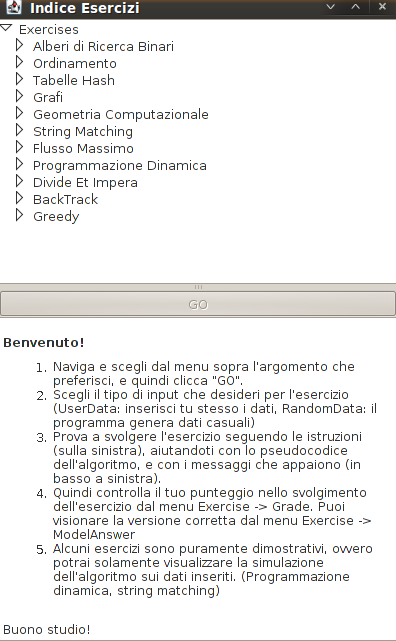
\includegraphics[scale=0.4]{images/Menu.png}
\caption{Menu iniziale}
\end{figure}


\section{\label{sec:Modifiche-apportate}Modifiche apportate}

E' stato scelto di sviluppare esclusivamente esercizi di simulazione
di algoritmi perchè in questo modo lo studente è il protagonista effettivo
dell'animazione. Il programma quindi non permette all'utente di realizzare
una propria animazione, in quanto questa funzione di MatrixPro non
è stata inclusa nel nuovo software. Questa scelta è stata presa per
due motivazioni: 
\begin{itemize}
\item i destinatari del programma sono studenti, non insegnanti, e quindi
si presuppone (in accordo con gli studi riportati nel capitolo \ref{capitolo1})
che siano più portati a utilizzare le visualizzazioni e sperimentarne
il comportamento attraverso l'inserimento di nuovi dati, piuttosto
che a creare nuove animazioni;
\item esistono già validi strumenti per la creazione di animazioni personalizzate,
come per l'appunto il software MatrixPro, che permettono di realizzarle
semplicemente anche in pochi minuti; l'obiettivo di questa tesi è
di realizzare qualcosa di nuovo e poco diffuso, piuttosto che creare
un programma già disponibile.
\end{itemize}
Inoltre, se si rendesse necessario, è possibile in un secondo momento
integrare il progetto al sistema MatrixPro in modo analogo a come
il sistema Trakla2 è stato unito a quest'ultimo.

Per realizzare al meglio un'applicazione semplice nell'uso, e soprattutto
interattiva, sono state apportate alcune modifiche ed estenzioni al
programma originale. Nelle prossime sezioni saranno analizzate in
dettaglio le variazioni.


\subsection{\label{sub:Tipologie-di-Esercizi}Tipologie di Esercizi}

Durante la realizzazione del progetto, si è osservato che per alcune
categorie di algoritmi la tecnica dell'esercizio di simulazione non
era adatta, in quanto l'esercizio risultava essere poco interessante
per l'utente poichè consisteva in un gran numero di operazioni da
eseguire tutte simili tra loro. L'esempio più rappresentativo di questa
problematica è la categoria degli algortimi di programmazione dinamica:
lo studente dovendo riempire con dei numeri una tabella (vedi esercizio
Longest Common Subsequence), perde interesse nell'argomento e non
approfondisce adeguatamente il problema e la sua soluzione.

Per questo motivo si è scelto di dividere la raccolta di problemi
in due sottoinsiemi: gli esercizi e le animazioni. Per la prima parte
si sono realizzati esercizi di simulazione molto simili a quelli forniti
da Trackla2, mentre per la seconda parte sono stati prodotte animazioni
dell'algoritmo, analoghe alla modalità {}``Model Answer'' degli
esercizi. Per le simulazioni, è stata quindi sacrificata un po' di
interattività a favore di una maggiore chiarezza dell'esercizio.


\subsection{\label{sub:Input-a-scelta}Input a scelta}

In accordo con i risultati degli studi di cui si parla nel capitolo
\ref{SCORRETTA:Ref: capitolo1}, è stata aggiunta al programma la
possibilità per l'utente di inserire dati in ingresso scelti personalmente.
Il software Trakla2 invece automaticamente generava un insieme di
dati casuali.

Questa nuova funzione garantisce un buon livello di interattività
dell'utente, con il minimo sforzo da parte di quest'ultimo: lo studente
può infatti inserire particolari dati per osservare il comportamento
dell'algoritmo nei casi limite. E' sempre comunque permesso l'utilizzo
di input casuali generati dal sistema.

La preferenza per una particolare tipologia di input avviene successivamente
alla scelta dell'esercizio: allo studente si presenta una finestra
in cui deve decidere se utilizzare i propri dati oppure farli generare
al programma. Se opta per l'input personalizzato, a seconda dell'esercizio
in analisi utilizzerà diversi tecniche per l'inserimento. In particolare
il diverso procedimento dipende dal tipo di struttura dati che utilizza
l'algoritmo. Il primo passo è comune alle tre tecniche: l'utente deve
inserire l'elenco delle chiavi (elementi di un vettore, nodi di un
grafo, nomi dei punti) all'interno di un campo di testo. In alcuni
casi non è previsto l'inserimento di queste chiavi, in quanto non
sono necessarie per la particolare simulazione. La dimensione dell'input
è definita implicitamente in questo passaggio. Il prossimo è invece
discriminante delle varie tecniche, e lo analizziamo nel dettaglio:
\begin{itemize}
\item Esercizi {}``normali'', in questa categoria rientrano tutti gli
esercizi che non utilizzano particolari strutture dati (grafi o aree
geometriche), e quindi principalmente contengono vettori e/o alberi.
Se l'esercitazione necessita solo di un elenco di valori-chiave con
i quali riempire la struttura, allora nessun'altra finestra viene
visualizzata, e lo studente passa direttamente all'attività di simulazione.
Se sono previsti dati aggiuntivi, come per esempio i parametri di
una funzione di hashing, si presenta una finestra in cui è possibile
inserire i valori di suddetti parametri aggiuntivi.
\item Grafi, la creazione di un grafo necessita di un elenco di nodi, ma
soprattutto della relazione di adiacenza tra questi. Nell'applicazione
l'inserimento di tale informazione è stato realizzato tramite una
matrice di adiacenza. Lo studente si trova di fronte ad una seconda
finestra, in cui è presentata una matrice costruita nel seguente modo:
le cui righe e colonne sono etichettate con i nodi precedentemente
inseriti, ed ogni elemento interno è un'area di testo (se il grafo
ha archi pesati) in cui si deve inserire il peso del relativo arco
(0 equivale a arco assente), oppure una casella di spunta per indicare
se esiste o meno un arco tra i due nodi. Se si sta parlando di un
grafo non orientato, è possibile inserire le informazioni della relazione
solo nella parte triangolare inferiore della matrice.
\item Geometria, per i due problemi di geometria computazionale è stato
creata una tecnica di input molto simile al primo tipo, in cui è possibile
inserire le coppie di coordinate (x,y) di ogni punto precedentemente
aggiunto.
\end{itemize}
Inizialmente era prevista anche un'ulteriore tipologia di inserimento
dati: i Test Cases {[}tradurre{]}. Essi prevedevano di fornire un
paricolare insieme di dati preparati dal programmatore (come suggerito
della guida \cite{wikiAlgoViz}) che permettessero allo studente di
osservare il comportamento dell'algoritmo in situazioni limite, poichè
egli potrebbe non avere l'intuizione corretta per realizzarle tramite
un input personalizzato. Successivamente questa possibilità è stata
accantonata per problemi di tempi nel completamento del progetto,
e per concentrarsi su altri aspetti dell'applicazione. L'inserimento
di tale funzione in un secondo momento non è comunque esclusa.


\subsection{Documentazione algoritmo}

Sono state fatte alcune integrazioni anche dal punto di vista dell'interfaccia
grafica del software, in particolare per la finestra di simulazione
degli esercizi, che sono descritte in questa e nelle due sezioni successive.

Per prima cosa è stato aggiunto un pannello laterale nella parte sinistra
della finestra, che contiene a sua volta tre pannelli tab {[}tabpanel..
come si traduce?{]}. In questa sezione analizzeremo due di questi
pannelli.

Il pannello {}``Descrizione'' contiene alcune informazioni dell'algoritmo,
in particolare una breve descrizione del problema affrontato, e le
istruzioni fondamentali per poter affrontare la simulazione nell'esercizio. 

Un secondo pannello contiene lo pseudo codice dell'algoritmo in questione,
ed è tratto dal libro \cite{libro}. In alcuni casi il codice di un
particolare problema non era presente su questo libro, e quindi si
riferisce ad un altro libro \cite{cormen}.

La gestione dei testi relativi ad ogni esercizio è stata realizzata
con l'aiuto di un file di testo esterno al codice, contenente tutte
queste proprietà. In questo modo si semplificano eventuali modifiche
future della documentazione, che non necessitano la compilazione del
codice sorgente, ma che consistono semplicemente in un aggiornamento
di questo file. Inoltre, si permette ad un potenziale docente che
utilizza un diverso testo per il proprio corso, di aggiornare i codici
e le informazioni degli algoritmi secondo le proprie preferenze.

La scelta di aggiungere questa sezione informativa al software è stata
fatta in seguito all'analisi degli altri programmi disponibili \ref{SCORRETTA:Ref: sec:Strumenti-Disponibili},
ma che JHAVE' \cite{JHAVE} il quale forniva allo studente una documentazione
sull'argomento come integrazione all'esercizio. Anche qui i testi
di sussidio non erano integrati nel codice, ma memorizzati in pagine
html {[}verificare{]}.


\subsection{\label{sub:Domande-relative-esercizio}Domande relative esercizio}

Un'altra funzionalità che è stata aggiunta al programma prendendo
spunto dalle caratteristiche di JAHVE' \cite{JHAVE}, è la possibilità
di confrontarsi con alcune domande a proposito dell'algoritmo o della
struttura dati analizzati. Nel programma JHAVE, l'animazione del problema
viene interrotta ponendo domande sull'argomento allo studente, con
una frequenza che varia a seconda di alcuni parametri impostati dal
programmatore. Lo studente per poter continuare l'animazione deve
rispondere alle domande che gli sono poste. Provando ad utilizzare
questo programma, alcuni studenti del corso di Informatica hanno trovato
fastidioso essere continuamente fermati nella presentazione da queste
domande. Nel nuovo progetto realizzato si è quindi optato per inserire
la possibilità di rispondere alle domande, ma a scelta dello studente.

Il pulsante per poter sottoporsi ad una domanda è posto nel terzo
pannello sulla sinistra, insieme ai due di cui si è parlato nelle
sezioni precedenti. Le domande, che variano da 3 a 5 per ogni esercizio,
sono di due tipologie: a scelta multipla o a risposta aperta (in cui
lo studente risponde scrivendo all'interno di un campo di testo),
e vengono visualizzate tramite una piccola finestra. Una volta inserita
la risposta, il programma comunica allo studente se è esatta o meno;
nel caso fosse sbagliata viene visualizzata la soluzione giusta. Le
domande e le loro risposte sono inserite direttamente nel codice di
ogni esercizio. Questo è sicuramente un punto debole, e quindi un
miglioramento futuro potrà trasportarle all'esterno del codice, magari
in un file di testo esterno, come per la documentazione degli esercizi.

E' stata inoltre sperimentata la possibilità di creare domande {}``dinamiche'',
ovvero che interagiscono direttamente con il contenuto dell'esercizio.
Per esempio in un esercizio di inserimento di dati in un albero di
ricerca binario, si potrebbe chiedere: {}``In quale nodo andrà inserita
la prossima chiave K'' {}``(Risposta) S''. In questo caso, sia
la domanda che la risposta, saranno modificate con i dati dell'esercizio,
sostituendo a K il valore della chiave che si è prossimi ad inserire
nella struttura, e a S il nome del nodo che diventerà padre di K.


\subsection{FeedBak RealTime}

I programmi di animazione di algoritmi sono usati spesso da studenti
alle prime armi con un determinato argomento, e che hanno bisogno
di vedere e toccare con mano per riuscire a focalizzare al meglio
il problema.s Uno studente non ferrato in un particolare algoritmo
non riuscirà a simulare correttamente già la prima volta l'esercizio,
e dovrà ricorrere continuamente alla funzione di Model Answer per
controllare se si sta muovendo correttamente nella struttura dati.
Per agevolare il primo apprendimento dell'argomento, si è quindi pensato
di aggiugere, sempre nella parte sinistra dello schermo, un'area di
testo che reagisce ai cambiementi effettuati dall'utente sulle strutture
dati, modificando il proprio testo e comunicando attraverso questo
allo studente se la simulazione di ogni passo è corretta. Per ogni
esercizio il criterio con cui si stabilisce se un particolare passo
è corretto, e il testo che di conseguenza deve apparire, sono diversi
e incorporati nel codice.

Per un utente esperto che vuole verificare le proprie conoscenze,
questa funzione può essere di disturbo: è stata perciò inserita la
possibilità di disattivare l'area di testo semplicemente un pulsante.
L'area può essere tuttavia riattivata in un secondo momento.


\section{\label{sec:Esempi}Esempi}

In questa sezione sono descritti due esercizi del programma, rappresentativi
delle due tipologie spiegate nella sezione \ref{sub:Tipologie-di-Esercizi}.
In particolare si analizza per la categoria degli esercizi di simulazione
l'Inserimento in un Albero Binario di Ricerca, e per la categoria
delle animazioni, il calcolo del numero di Fibonacci con la programmazione
dinamica.


\subsection{\label{sub:Inserimento-di-Chiavi}Inserimento di Chiavi in un Albero
Binario di Ricerca}

Lo studente, una volta scelto l'esercizio dall'elenco principale,
ha la possibilità di scegliere il metodo di inserimento dei dati che
preferisce. Come si è spiegato in \ref{sub:Input-a-scelta}, le opzioni
disponibili sono di inserire le informazioni, oppure di lasciare che
siano generate casualmente dal programma. Nel primo caso, l'utente
deve inserire in un campo di testo gli elementi che desidera inserire
nell'albero, che devono essere lettere separate da una virgola. Se
i dati inseriti non sono corretti (ad esempio una stringa vuota),
l'applicazione ripropone allo studente la finestra di scelta dell'input,
in modo che al momento della generazione dell'esercizio i dati siano
presenti e corretti.

L'utente si trova quindi di fronte alla finestra dell'esercizio vero
e proprio. Sulla sinistra dello schermo si trova il pannello laterale
contenente le funzioni aggiuntive descritte in \ref{sec:Modifiche-apportate}.
In questo esercizio l'area di testo dedicata ai messaggi del programma,
al momento è vuota, e in seguito conterrà il risultato della visita
in ordine dell'albero quando l'utente inserisce correttamente i nodi,
oppure un messaggio di errore {}``Attento!'' quando commette un
qualche sbaglio nell'inserimento.

Nella parte superiore è presente un pannello contenente quattro pulsanti
e una barra di scorrimento chiamato Animatore {[}controllare{]}, il
quale permette durante la simulazione dell'algoritmo di muoversi all'interno
dell'animazione creata fino a quel momento, concedendo anche l'opportunità
di modificare i passi precedenti.

Infine al centro della finestra si trova il pannello principale contenente
le strutture grafiche interattive, chiamato Structure Panel. In questo
esempio al suo interno si trovano un vettore contenente le chiavi
inserite in precedenza, e un albero al momento costituito solo da
un nodo vuoto. Come descritto del pannello {}``Descrizione'' a sinistra,
lo studente deve inserire nell'ordine in cui appaiono nel vettore,
le lettere all'interno dell'albero. La relazione di confronto tra
le chiavi è l'ordine alfabetico; se due chiavi hanno lo stesso valore,
la nuova va inserita alla destra di quella vecchia.

Per inserire le chiavi nell'albero è necessario cliccare su di esse
nel vettore e trascinarle nella posizione desiderata. Per facilitare
questa procedura, l'applicazione evidenzia con un colore rosso l'area
adatta al rilascio della chiave quando viene attraversata dal puntatore
del mouse. Se si commette qualche errore nell'inserimento, non si
deve trascinare nuovamente la chiave nel vettore: è necessario utilizzare
i comandi soprastanti di spostamento nell'animazione.

Quando si è terminata la simulazione si hanno a disposizione alcune
funzioni di controllo del proprio risultato fornite anche dal programma
originale, che sono {}``Grade'' che comunica quanti passaggi corretti
sono stati effettuati, {}``Model Answer'' che fornisce l'animazione
dell'algoritmo e {}``Compare'' che permette di confrontare passo
passo l'animazione prodotta dallo studente e quella corretta del programma,
sia in maniera sincrona che non.

\begin{figure}[htbp]
\centering
\includegraphics[scale=0.4]{images/ABR.png}
\caption{Inserimento in Albero Binario di Ricerca}
\end{figure} 


\subsection{Fibonacci}

L'esercizio del calcolo del numero di fibonacci contenuto nel programma,
è basato sulla tecnica della programmazione dinamica, ed è realizzato,
per le motivazioni espresse in \ref{sub:Tipologie-di-Esercizi}, come
un'animazione e non un esercizio.

Nonostante questo si ha, come per gli altri esercizi, la scelta di
usare un input casuale o di inserirlo personalmente. L'esercizio di
fibonacci prevede di ricevere come dato esterno solo un numero intero
maggiore di 0. Per questo, se lo studente sceglie di inserire lui
stesso i dati, non gli si presenterà la finestra per l'introduzione
delle chiavi, bensì quella dedicata all'immissione dei parametri integrativi.
In questa è presente solo un campo etichettato con il nome {}``n''
in cui si deve immettere il numero intero di cui si vuole calcolare
il relativo valore nella serie di Fibonacci.

La finestra dell'animazione che si presenta all'utente è molto simile
per struttura a quella degli esercizi come \ref{sub:Inserimento-di-Chiavi},
con la differenza che non è possibile interagire direttamente con
le strutture presenti nel pannello centrale. L'attività proposta infatti
non è altro che un'animazione classica, con alcune integrazioni, il
cui andamento può essere controllato dal pannello Animatore posto
nella parte superiore della finestra.

Nella parte centrale sono poste due strutture un vettore di un elemento
contenente il numero di Fibonacci inserito o generato dall'applicazione,
e un vettore al momento vuoto. Proseguendo nell'animazione si osserva
il funzionamento dell'algoritmo di programmazione dinamica (il cui
pseudocodice è presente del pannello laterale), il quale riempie l'array
un elemento alla volta con il relativo valore di Fibonacci. Il valore
contenuto nell'ultimo elemento è il numero di Fibonacci corrispondente
al numero inserito.

Al termine delle animazioni, non sono disponibili le funzioni model
answer e grade, in quanto non si è trattato di un esercizio vero e
proprio, ma solo di una dimostrazione. Le funzioni aggiunte \ref{sec:Modifiche-apportate}
sono invece attive: per esempio l'area di testo dedicata ai messaggi,
contiene ad ogni passaggio il calcolo del successivo elemento da inserire.

\begin{figure}[htbp]
\centering
\includegraphics[scale=0.4]{images/Fibonacci.png}
\caption{Animazione di Fibonacci}
\end{figure} 


\section{Implementazione, concetti base}

Il software MatrixPro, di cui sono disponibili i codici sorgente,
è scritto in codice Java e organizzato in numerosi pacchetti.

Gli esercizi non sono altro che una classe Java, che a seconda della
categoria a cui appartengono, implementano particolari interfacce
che ne definiscono le caratteristiche. Tutti gli esercizi per essere
tali devono definire almeno le procedure fondamentali come quelle
di inizializzazione, quelle per definire l'interazione dell'utente
con le strutture, e infine quelle per creare l'animazione risultato.

Le interfacce grafiche sono organizzate in maniera gerarchica a seconda
della loro funzione. La struttura principale che coinvolge gli esercizi
è lo Structure Panel, ovvero l'area centrale in cui sono presenti
le strutture dati dell'algoritmo. Il pannello gestisce l'aggiunta
e il comportamento di queste strutture, nonchè la loro visualizzazione.

Anche le strutture dati sono orgranizzate in modo gerarchico, sia
dal punto di vista del codice, che dalla presentazione che viene offerta
all'utente. Sono infatti suddivise in FDT (Fundamental Data Type)
e CDT (Conceptual Data Type), ovvero strutture primitive e strutture
astratte. Le prime sono tipi basilari come vettori, liste, grafi e
chiavi, e i comportamenti che consentono sono semplici assegnazioni
e modifiche dei collegamenti (per grafi e liste). I CDT invece consistono
in strutture più complesse per quanto riguarda la loro costruzione
e anche per i loro comportamenti. Un esempio di questa categoria è
la pila (Stack), realizzata a partire da un vettore, al quale sono
associate solo particolari operazioni (pop, push..). Le due diverse
categorie di strutture possono essere utilizzate allo stesso modo
senza problemi negli esercizi.

Un altro elemento fondamentale per la creazione delle animazione è
la classe {}``Animator''. Essa gestisce la memorizzazione dei passi
dell'animazione, e lo fa immagazzinando in uno stack gli stati delle
strutture interessate nella visualizzazione. E' questa classe che
gestisce lo spostamento all'interno dell'animazione. Essa inoltre
permette la valutazione tramite la funzione {}``Grade'' di un esercizio:
il risultato è dato infatti confrontando passo passo la simulazione
del programma e quella fornita dallo studente, entrambe memorizzate
in un animatore.

Lo sviluppo di nuovi esercizi consiste quindi nella programmazione
di nuove classi Esercizio, e nella realizzazione, se necessario, di
nuove strutture dati, progettate a partire da quelle già presenti
nell'applicazione.
